\documentclass[11pt]{article}
\usepackage[margin=1in]{geometry}
\usepackage{graphicx}
\usepackage{booktabs}
\usepackage{amsmath}
\usepackage{hyperref}
\usepackage{caption}
\hypersetup{colorlinks=true, linkcolor=blue, citecolor=blue, urlcolor=blue}

\title{Healing AI Amnesia in Physics-Informed Neural Networks:\\
\large A 47.6\% Accuracy Fix for PINN Retraining via Optimizer State Preservation}
\author{Harshit Lalwani}
\date{}

\begin{document}
\maketitle

\begin{abstract}
Physics-Informed Neural Networks (PINNs) are commonly retrained in phases --- e.g., an initial fit
followed by one or more fine-tuning passes --- and it is standard practice to reinitialize the Adam
optimizer at the start of each phase. This reset is a bug, not a neutral default: it silently discards
the optimizer's accumulated gradient-moment estimates, and on the 1D Fisher--KPP reaction--diffusion
equation it makes every successive retraining phase \emph{worse}, with relative $L_2$ error against the
analytical traveling-wave solution rising monotonically from $5.01\times10^{-2}$ to $8.70\times10^{-2}$.
\textbf{The fix is simple: don't reset it.} Preserving Adam's internal moment estimates across phases
(and, for a final fine-tuning phase, switching to L-BFGS with its own state likewise preserved) reverses
this entirely --- error instead falls monotonically, from $5.82\times10^{-2}$ to $4.56\times10^{-2}$ ---
a $\mathbf{47.6\%}$ reduction in final error relative to the reset baseline, turning retraining from
actively harmful into actively helpful. This bug and its fix were identified but never implemented or
quantified by Aberqi \& Miloudi \cite{aberqi2026fisher}, whose Section 5.2 only recommends the fix in
passing; we implement it and measure its effect directly. We additionally test whether the fix
generalizes by extending to the 2D Fisher--KPP equation, which the source paper does not address, via a
32-configuration sweep over network width/depth and learning-rate schedule; there we find a genuine
negative result along a different axis: a wider, shallower $6\times100$ architecture diverges on every
configuration tested ($L_2 \approx 1.0$), while a narrower, deeper $7\times50$ architecture converges
reliably ($L_2 = 0.023 \pm 0.006$) in less training time.
\end{abstract}

\section{The Bug and the Fix}

Retraining a neural network in phases is routine: fit once, then fine-tune, often more than once, as
more data or compute becomes available. For a PINN, each phase minimizes the same composite
physics-informed loss, just resumed from the previous phase's weights. What is \emph{not} routine to
get right is what happens to optimizer state at that resumption point. The default --- construct a new
optimizer for each phase --- silently throws away Adam's running estimates of each parameter's gradient
mean and variance, the state it uses to adapt its effective per-parameter step size. On the Fisher--KPP
problem studied here, that default is actively harmful: every retraining phase makes the model worse,
not better (Section~\ref{sec:results}, Table~\ref{tab:1d-results}).

The fix tested in this work is direct: save the optimizer's state dictionary at the end of one phase and
load it back before the next, so retraining resumes the same optimization trajectory rather than
restarting it under a colder, less-adapted state. We validate this fix on the 1D Fisher--KPP equation
from Aberqi \& Miloudi \cite{aberqi2026fisher} --- whose own experiments exhibit the reset bug and whose
Section 5.2 recommends this exact fix without implementing or quantifying it --- and then test whether
the fix's benefit is specific to that 1D setup or generalizes, by repeating the same reset-vs-preserved
comparison on an original 2D extension of the same equation.

\section{Background}

The Fisher--KPP equation,
\begin{equation}
u_t = D\,u_{xx} + R\,u\,(1-u),
\end{equation}
is a reaction--diffusion PDE with a well-known analytical traveling-wave solution, which makes it a
convenient testbed for evaluating PINN training methodology against ground truth rather than only
against a numerical baseline. Aberqi \& Miloudi \cite{aberqi2026fisher} use exactly this equation as
their testbed, training a PINN in three phases (an initial 10k-iteration Adam run, followed by two
20k-iteration Adam retraining phases) and reporting that accuracy degrades with each successive
retraining phase. Their Section~5.2 attributes this to the optimizer-reset bug described above and
recommends, without implementing or quantifying it, the fix this work tests.

\section{Method}

\subsection{Shared PINN setup}

Both the 1D reset and 1D state-preserving experiments use the same architecture: a fully-connected
network with 7 hidden layers of 50 tanh units, Xavier-normal weight initialization and zero bias
initialization, mapping $(x,t) \mapsto u(x,t)$. The training loss is the standard PINN composite,
\begin{equation}
\mathcal{L} = \lambda_{\text{IC}} \mathcal{L}_{\text{IC}} + \lambda_{\text{BC}} \mathcal{L}_{\text{BC}}
+ \lambda_{\text{Res}} \mathcal{L}_{\text{Res}},
\end{equation}
evaluated over 10{,}000 interior collocation points, 1{,}000 initial-condition points ($t=0$), and
2{,}000 boundary-condition points ($x \in \{0,1\}$), with $\mathcal{L}_{\text{Res}}$ the mean-squared
PDE residual computed via automatic differentiation. The IC/BC weights follow the paper's adaptive
scheme, ratcheting monotonically toward a cap based on the ratio of the residual loss to the IC/BC
loss, while $\lambda_{\text{Res}}$ stays fixed at 1.0. Training proceeds in three phases and accuracy is
reported as the relative $L_2$ error against the exact traveling-wave solution on a held-out grid.

\subsection{Reset vs.\ state-preserving retraining}

The two conditions differ only in what happens to optimizer state at each phase boundary:

\begin{itemize}
\item \textbf{Reset (paper-faithful baseline, \texttt{pinn\_early.ipynb}):} at the start of every phase
a fresh \texttt{torch.optim.Adam} is constructed, discarding all first- and second-moment estimates
accumulated in the previous phase. This matches the source paper's own protocol.
\item \textbf{State-preserving (\texttt{memoryAwarePINN/modiified\_pinn.ipynb}):} the model weights and
the optimizer's moment estimates both carry over between phases. Phase~1 and Phase~2 use Adam with its
state dictionary preserved across the boundary; Phase~3 switches to L-BFGS, with its own state saved
and restored, as a further fine-tuning step once the Adam phases have converged.
\end{itemize}

All other hyperparameters (learning rate schedule, iteration counts per phase, collocation/IC/BC point
counts, network architecture) are held fixed between the two conditions so that optimizer-state handling
is the only varied factor.

\subsection{2D extension}

The 2D Fisher--KPP problem extends the domain to $(x,y) \in [0,1]^2$, with initial and boundary
conditions sampled analogously (1{,}000 initial points, 4{,}000 boundary points across the four domain
edges, 10{,}000 collocation points). We sweep 32 configurations crossing two architectures
($7\times50$ and $6\times100$, tanh) with different Phase-1/Phase-2 learning-rate schedule combinations
(cosine, linear, exponential, and delayed-exponential decay), each run through the same three-phase
protocol and evaluated by final relative $L_2$ error and wall-clock training time.

\section{Results}
\label{sec:results}

\subsection{1D: state preservation reverses the direction of retraining}

Table~\ref{tab:1d-results} reports the relative $L_2$ error at the end of each phase for both
conditions, read directly from the executed notebooks' printed output.

\begin{table}[h]
\centering
\caption{1D Fisher--KPP relative $L_2$ error by phase. Phase~3 for the state-preserving run uses
L-BFGS; all other phases use Adam.}
\label{tab:1d-results}
\begin{tabular}{lccc}
\toprule
Condition & Phase 1 & Phase 2 & Phase 3 (final) \\
\midrule
Optimizer reset each phase (paper protocol) & $5.01\times10^{-2}$ & $7.69\times10^{-2}$ & $8.70\times10^{-2}$ \\
Optimizer state preserved & $5.82\times10^{-2}$ & $4.55\times10^{-2}$ & $4.56\times10^{-2}$ \\
\bottomrule
\end{tabular}
\end{table}

With the optimizer reset every phase, error rises monotonically with each retraining pass, degrading by
$73.6\%$ from Phase~1 to Phase~3 --- consistent with the source paper's own reported degradation from
resetting Adam state. With optimizer state preserved, error instead falls monotonically, improving by
$21.6\%$ from Phase~1 to Phase~3. The final head-to-head comparison is
$8.70\times10^{-2}$ (reset) vs.\ $4.56\times10^{-2}$ (preserved) --- a $\mathbf{47.6\%}$ reduction in
final error, and a complete reversal of whether retraining helps or hurts. Figure~\ref{fig:1d-summary}
visualizes this reversal directly.

\begin{figure}[h]
\centering
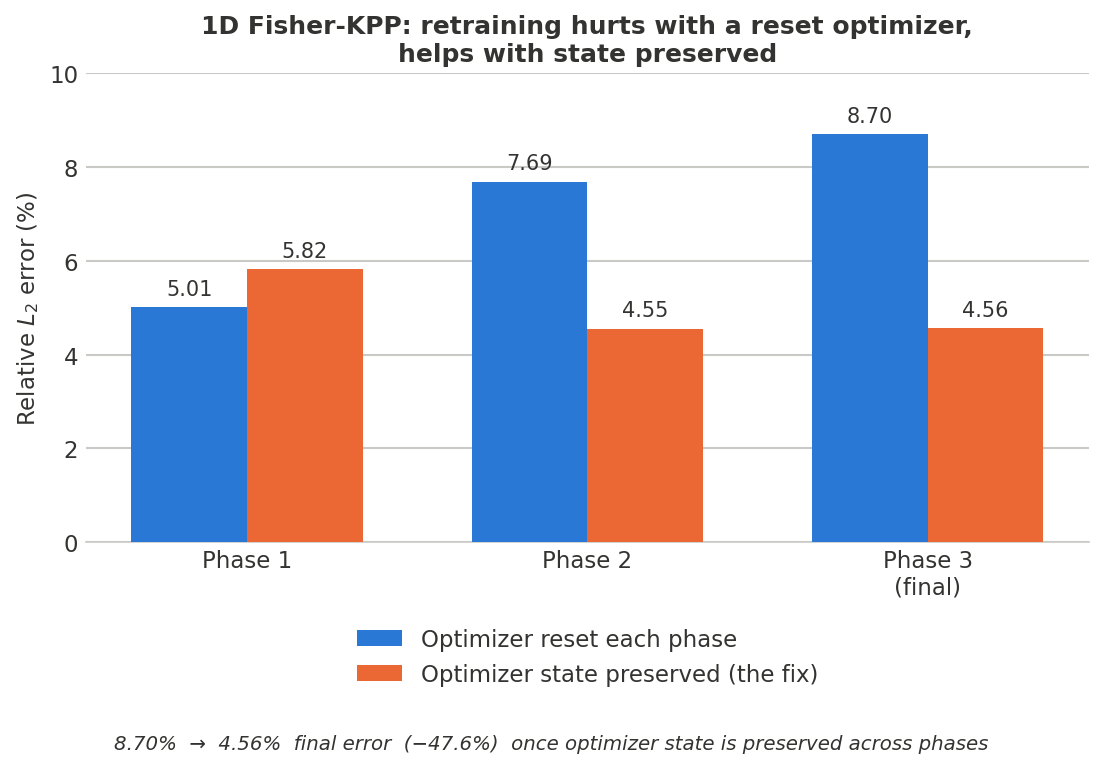
\includegraphics[width=0.75\textwidth]{../figures_summary/1d_reset_vs_preserved.png}
\caption{Relative $L_2$ error by retraining phase: the reset condition (the bug) gets worse every
phase; the state-preserved condition (the fix) gets better every phase.}
\label{fig:1d-summary}
\end{figure}

Figure~\ref{fig:1d-reset} shows the full training history (loss, adaptive weights, and $L_2$ error vs.\
iteration) for the reset condition; Figure~\ref{fig:1d-preserved} shows the same for the
state-preserving condition. Both are the diagnostic plots produced directly by each notebook's own
training loop, unmodified.

\begin{figure}[h]
\centering
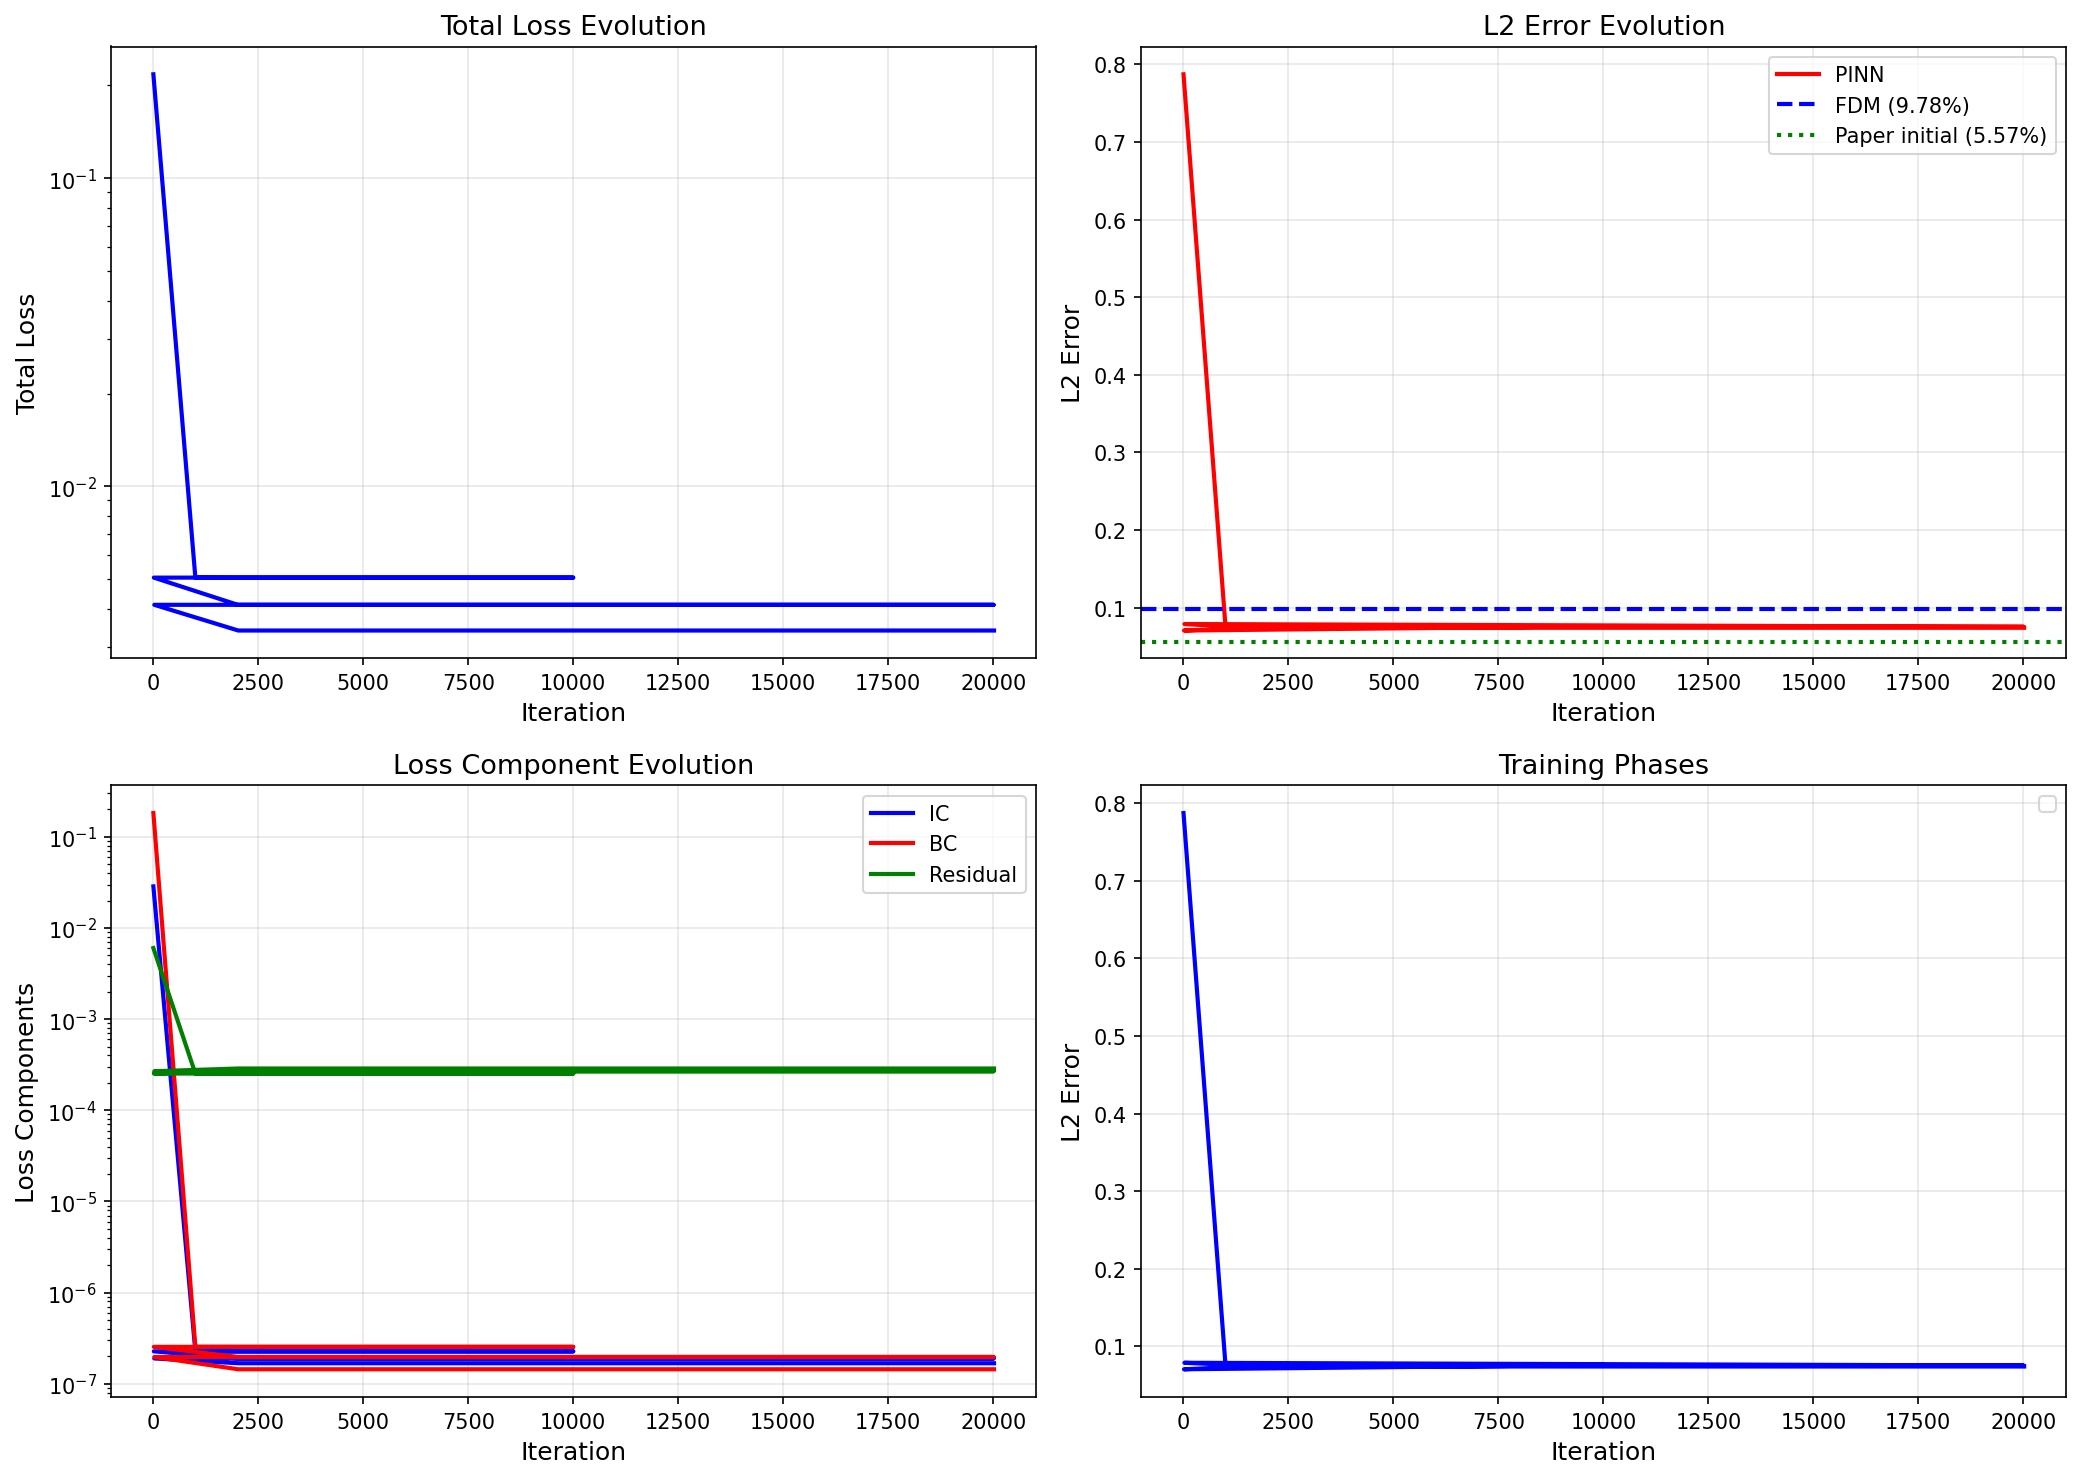
\includegraphics[width=0.92\textwidth]{../results/1d/pinn_training_history.png}
\caption{1D Fisher--KPP training history with the optimizer reset at each phase boundary
(\texttt{pinn\_early.ipynb}). $L_2$ error rises across phases.}
\label{fig:1d-reset}
\end{figure}

\begin{figure}[h]
\centering
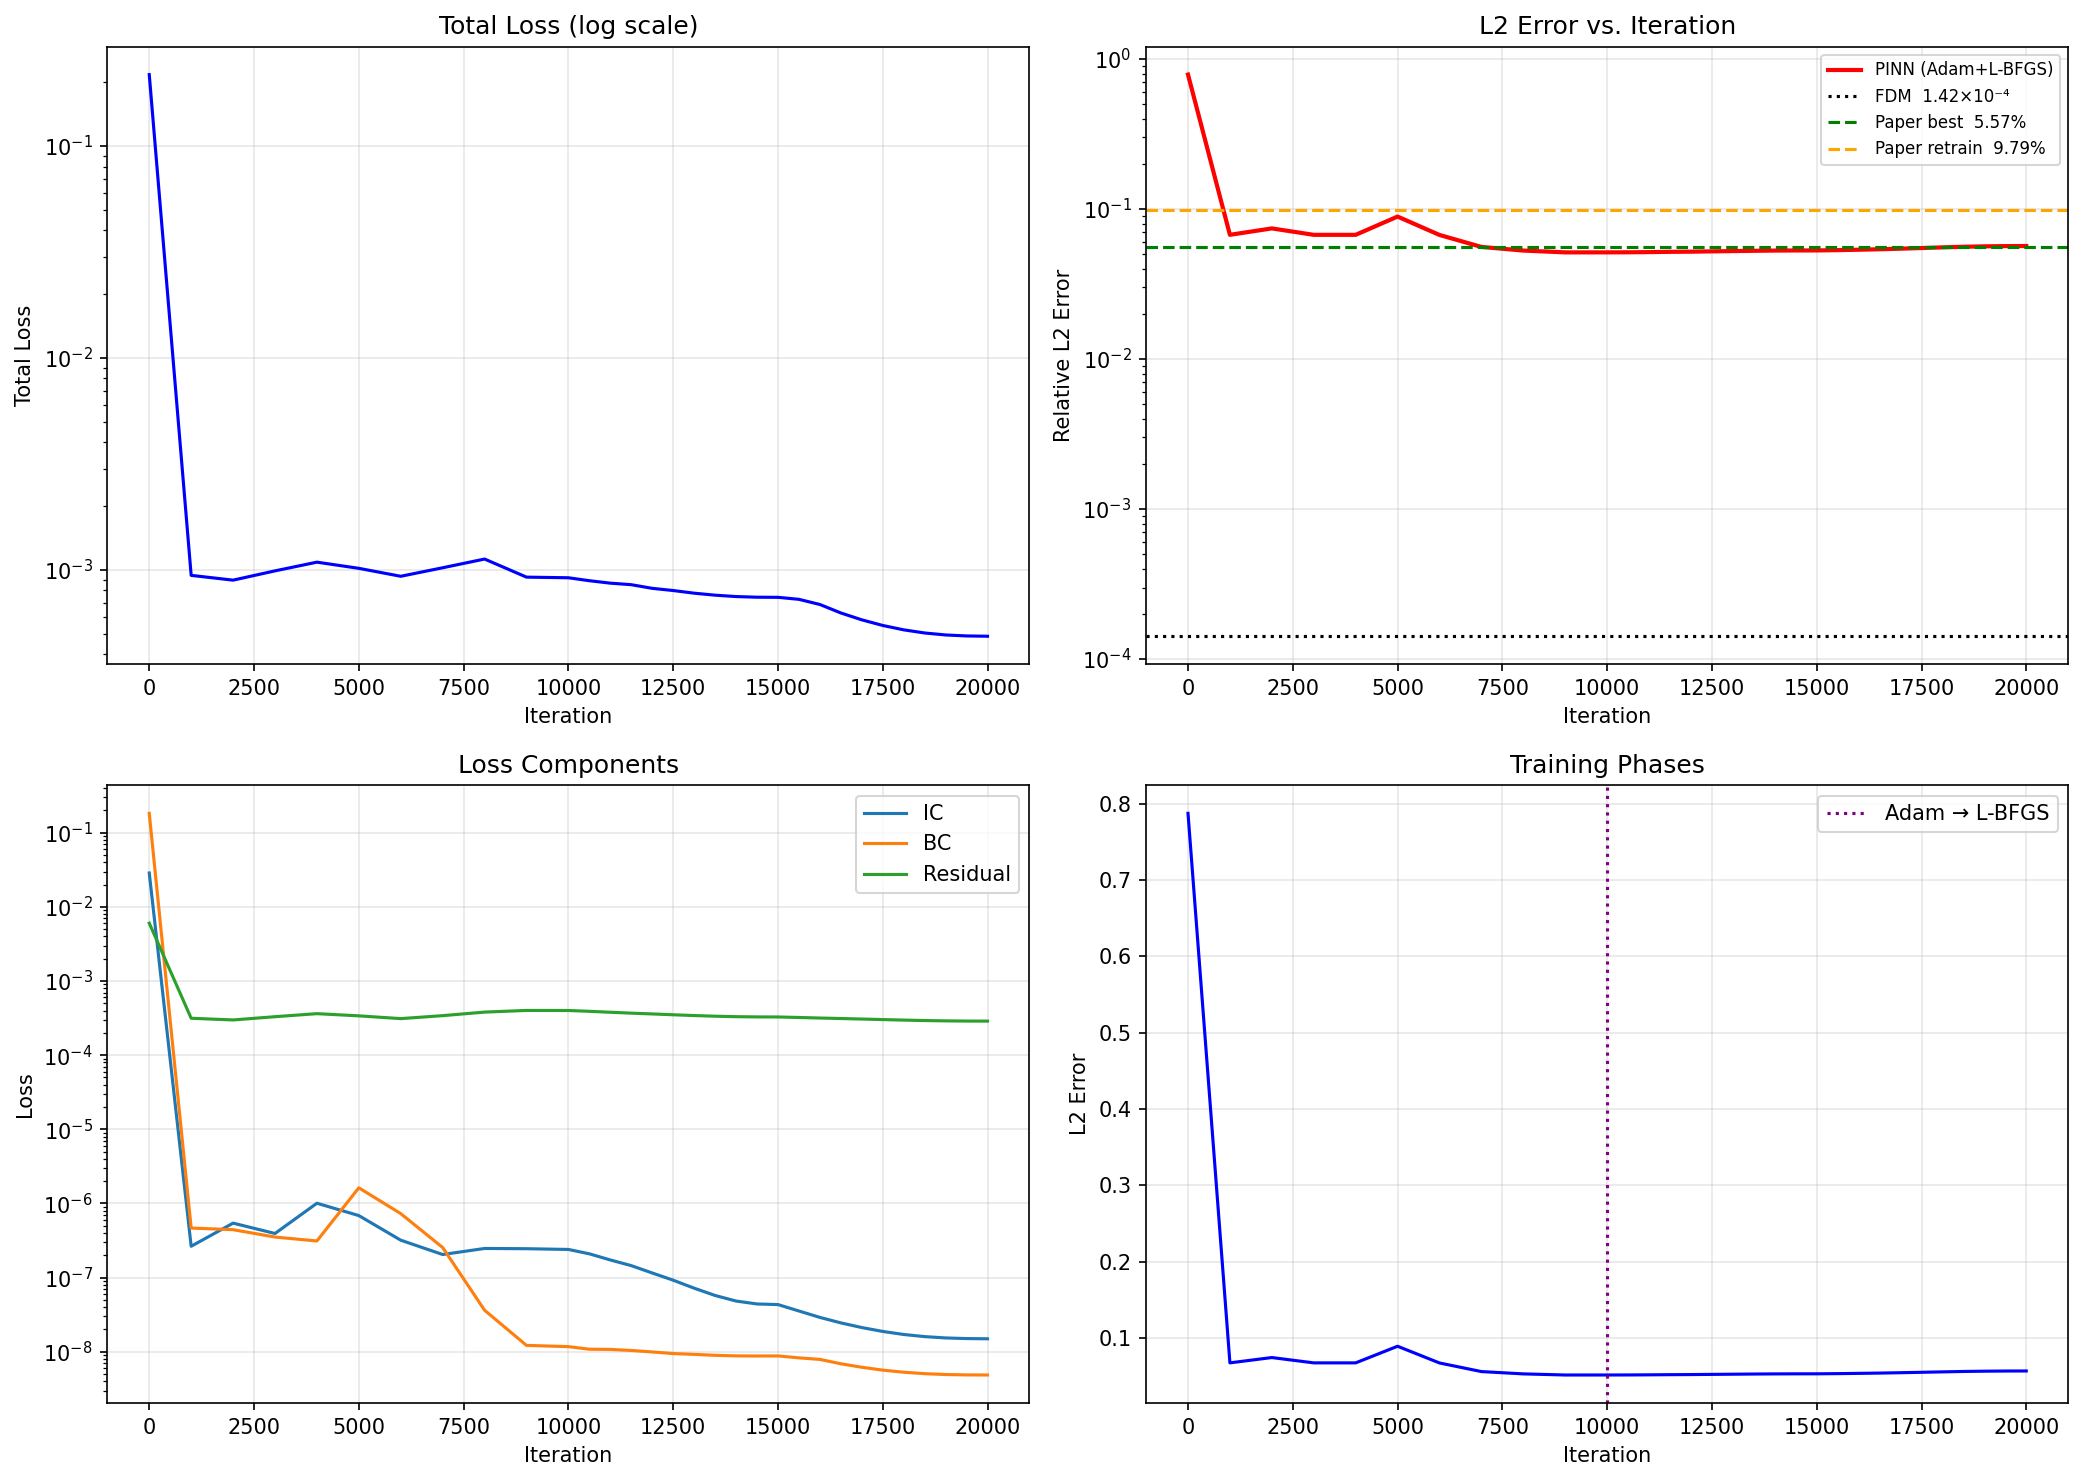
\includegraphics[width=0.92\textwidth]{../results/1d/training_history_lbfgs.png}
\caption{1D Fisher--KPP training history with optimizer state preserved across phases
(\texttt{memoryAwarePINN/modiified\_pinn.ipynb}), Phase~3 using L-BFGS. $L_2$ error falls across
phases.}
\label{fig:1d-preserved}
\end{figure}

\subsection{2D: does the fix generalize? Architecture, not just optimizer handling, matters}

Across the 32-configuration sweep (\texttt{results/2d/sweep/sweep\_results\_2d\_32.csv}), the two
architectures produce starkly different outcomes regardless of learning-rate schedule, summarized in
Table~\ref{tab:2d-results} and Figure~\ref{fig:2d-summary}.

\begin{table}[h]
\centering
\caption{2D Fisher--KPP results by architecture, aggregated over all 16 schedule configurations per
architecture (mean $\pm$ std.\ over final-phase relative $L_2$ error and training time).}
\label{tab:2d-results}
\begin{tabular}{lcc}
\toprule
Architecture & Final $L_2$ error & Training time (min) \\
\midrule
$7\times50$ & $0.023 \pm 0.006$ & $2.31 \pm 0.04$ \\
$6\times100$ & $1.000 \pm 0.0001$ & $4.23 \pm 0.01$ \\
\bottomrule
\end{tabular}
\end{table}

\begin{figure}[h]
\centering
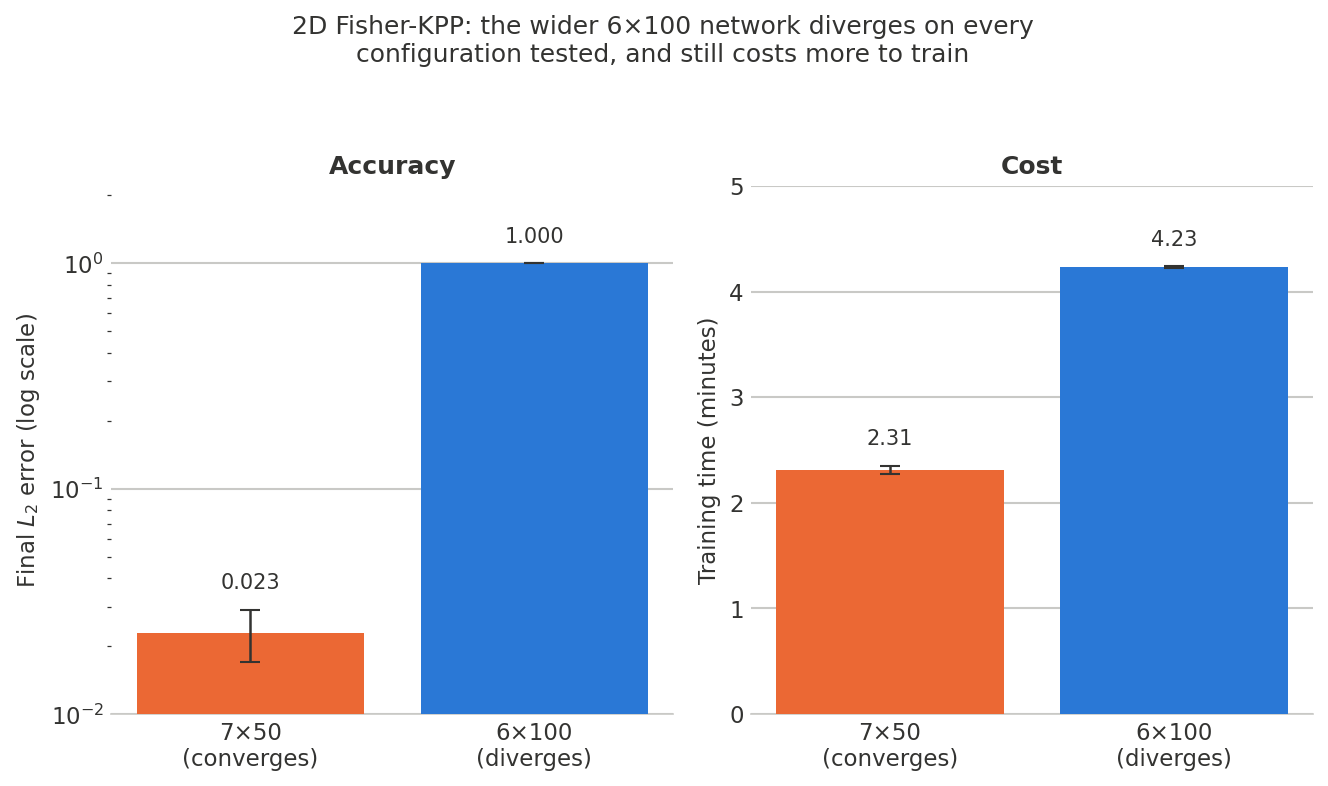
\includegraphics[width=0.85\textwidth]{../figures_summary/2d_architecture_comparison.png}
\caption{2D Fisher--KPP: final $L_2$ error (log scale, left) and training time (right) by
architecture, mean $\pm$ std.\ over the 16 schedule configurations per architecture.}
\label{fig:2d-summary}
\end{figure}

The $7\times50$ network converges on every one of the 16 schedule configurations tested. The
$6\times100$ network diverges on all 16 --- $L_2 \approx 1.0$ indicates the network has collapsed to a
trivial (near-constant) solution rather than fitting the traveling wave --- and, despite failing to
converge, still takes $83\%$ longer to train per run than the architecture that does converge.
Figure~\ref{fig:2d-collapse} visualizes this architecture collapse directly.

\begin{figure}[h]
\centering
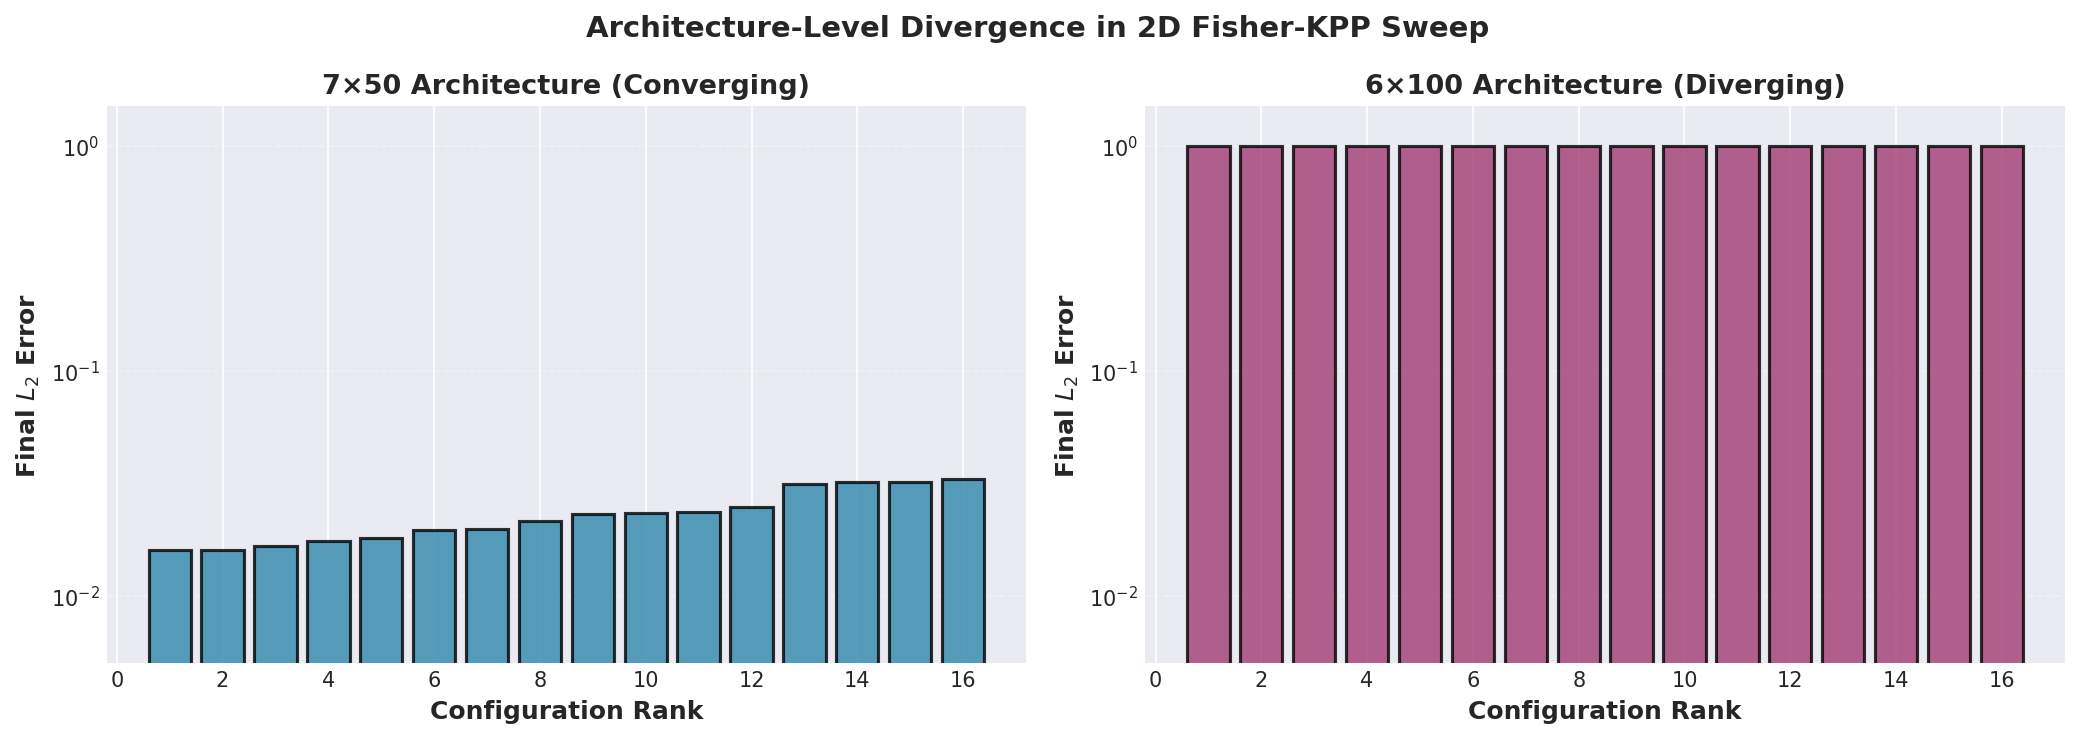
\includegraphics[width=0.95\textwidth]{../figures_2d/graph_1_architecture_collapse.png}
\caption{2D Fisher--KPP: the $7\times50$ architecture converges across all 16 sweep configurations
(left) while the $6\times100$ architecture diverges on all 16 (right).}
\label{fig:2d-collapse}
\end{figure}

\section{Discussion}

\textbf{Why does preserving optimizer state help?} The notebooks' own printed diagnostics attribute the
reset condition's degradation to Adam's accumulated first- and second-moment estimates being discarded
at each phase boundary --- consistent with the source paper's Section~5.2 root-cause explanation.
Those moments encode a running estimate of each parameter's gradient mean and variance, which Adam uses
to scale its effective per-parameter step size; discarding them forces the optimizer to re-estimate this
scaling from scratch under a new (smaller) learning rate, which this experiment's results are consistent
with degrading rather than refining the Phase~1 solution. Preserving that state lets later phases behave
as a continuation of the same optimization trajectory instead of a fresh, colder start, which the
monotonic \emph{improvement} across phases in the preserved condition supports directly.

\textbf{Why does the wider 2D architecture fail?} This is a genuinely open question --- the sweep
results establish the failure mode (collapse to $L_2\approx1$ on every configuration, independent of
learning-rate schedule) but the repository does not contain code or notebook analysis that isolates a
mechanism, so no root cause is claimed here beyond the observation that width traded for depth
($6\times100$ vs.\ $7\times50$) is both slower and consistently fails to converge on this 2D problem.

\section{Relationship to prior work}

The bug this work fixes --- and the 1D setup used to test the fix --- both come from Aberqi \&
Miloudi \cite{aberqi2026fisher}: their three-phase training protocol, architecture, and evaluation
methodology are used here largely as-is, and the reset-condition numbers in Table~\ref{tab:1d-results}
track that paper's own reported per-phase degradation pattern. The paper itself only
\emph{recommends} saving and restoring optimizer state (Section~5.2) as a plausible fix; it does not
implement or quantify that fix. This work's contribution on the 1D side is implementing that fix and
measuring its effect directly against the paper's own baseline, yielding the $47.6\%$ final-error
reduction reported above. The 2D extension is original in full: the source paper is 1D only, and the
architecture/schedule sweep, its failure mode, and its quantification have no counterpart in the source
paper.

\section{Conclusion}

Resetting the Adam optimizer at each retraining phase boundary is a common default, not a neutral one:
on the 1D Fisher--KPP PINN studied here (and, per Aberqi \& Miloudi \cite{aberqi2026fisher}, in the
source paper's own experiments) it causes accuracy to degrade with every retraining pass. The fix ---
preserving optimizer state across phases instead of resetting it --- reverses this entirely, turning
retraining from harmful to helpful and reducing final relative $L_2$ error by $47.6\%$. Testing whether
this generalizes, a 2D extension of the same problem surfaces a second, independent effect: architecture
choice can dominate optimizer-handling entirely, with a wider $6\times100$ network failing to converge
under any tested schedule while a narrower, deeper $7\times50$ network converges reliably and trains
faster.

\begin{thebibliography}{9}
\bibitem{aberqi2026fisher}
Aberqi, A. \& Miloudi, Y. \emph{Solving the Fisher Nonlinear Differential Equations via PINNs: A
Comprehensive Retraining Study and Comparative Analysis with the Finite Difference Method}.
arXiv:2601.11406v1.
\end{thebibliography}

\end{document}
